\documentclass[10pt,twocolumn]{article}
\usepackage[utf8]{inputenc}
\usepackage[T1]{fontenc}
\renewcommand{\figurename}{Figura}\renewcommand{\tablename}{Tabela}\renewcommand{\refname}{Referências}\renewcommand{\contentsname}{Sumário}
\usepackage{charter}
\usepackage[a4paper,margin=1.9cm,top=2.0cm,bottom=2.0cm,columnsep=0.7cm]{geometry}
\usepackage[authoryear,round]{natbib}
\usepackage{booktabs,multirow,graphicx,amsmath,amssymb,xcolor,fancyhdr,titlesec,caption,url,microtype,setspace}
\usepackage[colorlinks=true,linkcolor=blue!50!black,citecolor=blue!50!black,urlcolor=blue!50!black]{hyperref}
\captionsetup{font=footnotesize,labelfont=bf,skip=3pt}
\setlength{\bibsep}{0pt}\setlength{\parindent}{1.1em}\setlength{\parskip}{0pt}
\titleformat{\section}{\bfseries\normalsize}{\thesection.}{0.5em}{}
\titleformat{\subsection}{\itshape\normalsize}{\thesubsection.}{0.5em}{}
\titlespacing*{\section}{0pt}{9pt}{4pt}\titlespacing*{\subsection}{0pt}{6pt}{2pt}
\pagestyle{fancy}\fancyhf{}
\fancyhead[L]{\footnotesize\textit{Finanças do Setor Público (CCA0169) --- UnB --- P2, 2026.2}}
\fancyhead[R]{\footnotesize Matrícula 211014396}
\fancyfoot[C]{\footnotesize\thepage}
\renewcommand{\headrulewidth}{0.4pt}
\newcommand{\ep}[1]{{\scriptsize(#1)}}
\hypersetup{pdftitle={Transferências intergovernamentais, efeito flypaper e esforço fiscal: Tabatinga, Humaitá e Malásia},pdfauthor={Matrícula 211014396}}

\begin{document}
\twocolumn[{
\begin{@twocolumnfalse}
\vspace{2pt}
{\LARGE\bfseries Transferências intergovernamentais, efeito flypaper e esforço fiscal local: Tabatinga e Humaitá (AM) frente ao Amazonas e à Malásia, 2014--2023\par}
\vspace{8pt}
{\large Matrícula 211014396}\par
\vspace{3pt}
{\footnotesize Universidade de Brasília (UnB) --- Finanças do Setor Público, CCA0169, Turma 01, 2026.2 --- Prof. Lucas Oliveira Gomes Ferreira}\par
\vspace{6pt}\hrule\vspace{6pt}
\noindent\begin{minipage}[t]{0.27\textwidth}\footnotesize
\textbf{I N F O R M A Ç Ã O}\par\vspace{3pt}\hrule\vspace{3pt}
\textit{Histórico:}\\ Versão de 23 de outubro de 2026\\ Entrega (P2): 25 de outubro de 2026\par\vspace{3pt}\hrule\vspace{3pt}
\textit{Classificação JEL:}\\ H71, H72, H77, C23\par\vspace{3pt}\hrule\vspace{3pt}
\textit{Palavras-chave:}\\ Transferências intergovernamentais\\ Efeito flypaper\\ Ilusão fiscal\\ Esforço fiscal local\\ Dados em painel
\end{minipage}\hfill
\begin{minipage}[t]{0.69\textwidth}\small
\textbf{R E S U M O}\par\vspace{3pt}\hrule\vspace{3pt}
\noindent Os 62 municípios do Amazonas obtêm, em mediana, cerca de 95\% da receita total de transferências. O artigo atualiza e amplia a base do trabalho anterior (P1) com dados do Siconfi/Finbra e do IBGE para 2014--2023, em reais de 2023 e \textit{per capita}, e estima, em painel com efeitos fixos de município e de ano, como o gasto corrente e a receita própria respondem às transferências. Tabatinga e Humaitá são os casos focais; a Malásia entra como contraponto institucional, com dados do Banco Mundial e do FMI. A elasticidade do gasto corrente às transferências (0,53) é cerca de três vezes a elasticidade ao PIB \textit{per capita} (0,18), padrão compatível com o efeito flypaper, e o resultado se mantém sem o FUNDEB e sem os dois municípios focais. O gasto sobe com aumentos das transferências (0,21), mas a resposta às quedas não é distinguível de zero; a diferença entre as duas respostas, contudo, não é estatisticamente significativa (p = 0,17). Não há evidência de substituição de receita própria por transferências. Os resultados são associações condicionais, não efeitos causais. O referencial se apoia em 80 artigos de periódicos recuperados no Scopus e mapeados com análise bibliométrica.
\par\vspace{4pt}\noindent{\footnotesize\textbf{Abstract.} Amazonas' 62 municipalities obtain a median of about 95\% of total revenue from transfers. Using updated Siconfi/Finbra and IBGE data for 2014--2023 (2023 reais, per capita), we estimate two-way fixed-effects panels of current spending and own revenue on intergovernmental transfers, with Tabatinga and Humaitá as focal cases and Malaysia as an institutional benchmark. The spending elasticity to transfers (0.53) is about three times that to per capita GDP (0.18), consistent with a flypaper effect that survives dropping FUNDEB and the focal municipalities. Spending rises when transfers rise (0.21) but the response to cuts is statistically indistinguishable from zero, although the difference between both responses is not significant (p = 0.17). We find no evidence that transfers displace own revenue. Results are conditional associations, not causal effects.}
\end{minipage}
\vspace{6pt}\hrule\vspace{10pt}
\end{@twocolumnfalse}
}]

\section{Introdução}
Em 2023, Tabatinga recebeu R\$ 4,4 mil por habitante em transferências (valores de 2023), cerca de 92\% de sua receita total; Humaitá, R\$ 3,7 mil, ou 87\%. Em ambos, a arrecadação tributária própria respondeu por 4\% e 7\% da receita. Esses municípios são típicos do Amazonas, onde a mediana de dependência de transferências ficou entre 95\% e 96\% em todos os anos de 2014 a 2023. Nesse arranjo, o que o município gasta depende sobretudo do que o governo federal e o estadual repassam, e a pergunta clássica da federação fiscal ganha peso: o dinheiro que chega como transferência é gasto de forma diferente do dinheiro que nasce da renda local?

A literatura chama de \textit{efeito flypaper} a observação de que transferências de montante fixo estimulam mais gasto local do que aumentos equivalentes da renda privada \citep{hamilton1983,bailey1998}. A explicação mais antiga é a ilusão fiscal, em que eleitores subestimam o custo dos serviços financiados por recursos de fora \citep{dollery1996,turnbull1998}. Explicações concorrentes, que dispensam a ilusão, incluem o custo marginal dos fundos públicos \citep{hamilton1986,dahlby2011}, a pressão de grupos de interesse \citep{dougan1988} e o seguro contra incerteza \citep{vegh2015}. Para o Brasil, \citet{ferreira2019} encontram flypaper em 476 municípios entre 2005 e 2012, e \citet{ferreiralog2021} desenvolve o tema para as transferências constitucionais; o presente artigo segue essa linha.

\textbf{Contribuição.} Este é o produto 2 (P2) da disciplina: atualiza e amplia a base do P1 e produz o artigo. O repositório do P1 não continha dados utilizáveis para as unidades desta atribuição (Tabatinga, Humaitá e Malásia), e a base foi reconstruída a partir de fontes oficiais (seção~\ref{sec:dados}). Os ganhos são três: (i) painel de 62 municípios do Amazonas em 10 anos, que dá poder estatístico onde dois municípios dariam menos de 20 observações; (ii) tratamento explícito das três mudanças do plano de contas de receitas do Siconfi no período; (iii) contraste com a Malásia, tratado como comparação institucional e não como amostra conjunta.

\textbf{Estrutura.} A seção~\ref{sec:biblio} mapeia a literatura. A seção~\ref{sec:teoria} apresenta o referencial e as hipóteses. A seção~\ref{sec:dados} descreve dados e modelos. A seção~\ref{sec:res} traz os resultados e a seção~\ref{sec:conc} conclui.

\section{Mapeamento bibliométrico}\label{sec:biblio}
A base de literatura veio do Scopus, acessado pelo Portal de Periódicos da CAPES em 23/10/2026, com busca nos títulos, resumos e palavras-chave por \textit{flypaper effect}, \textit{fiscal illusion}, \textit{intergovernmental transfers} e \textit{intergovernmental grants}. A exportação trouxe 1.083 documentos. Com o pacote \textit{bibliometrix} (R 4.6.1; \texttt{convert2df}, \texttt{biblioAnalysis}, \texttt{biblioNetwork} e \texttt{thematicMap}; \textit{script} \texttt{R/05\_bibliometrix.R}), mantidos artigos e revisões de periódico, a análise cobre 968 documentos, de 1952 a 2026 (o ano de 2026 está incompleto), em 397 periódicos, com 1.588 autores e média de 19,0 citações por documento.

A produção cresce de menos de 20 trabalhos por ano até a década de 1990 para um patamar de 40 a 55 por ano desde 2017 (painel A). Os Estados Unidos concentram a produção (cerca de 125 documentos), seguidos por Espanha, China, Índia e Reino Unido, com o Brasil em sexto; o Reino Unido e a Itália têm participação alta de coautorias internacionais (painel B). Dois periódicos concentram a literatura, \textit{Public Choice} (60) e \textit{Public Finance Review} (51), seguidos por \textit{International Tax and Public Finance} (30), \textit{Journal of Public Economics} (29) e \textit{European Journal of Political Economy} (24). A palavra-chave mais frequente é \textit{intergovernmental transfers} (192), à frente de \textit{intergovernmental grants} (95), \textit{fiscal federalism} (82), \textit{flypaper effect} (66) e \textit{fiscal illusion} (65). A rede de co-ocorrência (painel C) liga \textit{flypaper effect} e \textit{fiscal illusion} ao núcleo \textit{intergovernmental transfers/grants} e \textit{fiscal federalism}. No mapa temático (painel D), \textit{intergovernmental transfers}, \textit{fiscal federalism} e \textit{political economy} formam o tema básico; \textit{fiscal illusion}, \textit{local government} e \textit{fiscal policy} aparecem como tema motor; e \textit{intergovernmental grants}, \textit{flypaper effect} e \textit{fiscal capacity} ficam no quadrante de temas emergentes ou em declínio, o que indica espaço para estudos sobre esforço fiscal local. Há poucos trabalhos sobre a Malásia: a base não contém nenhum artigo sobre transferências a governos subnacionais malaios, o que limita a parte comparativa e é discutido na seção~\ref{sec:conc}.

\begin{figure*}[t]
\centering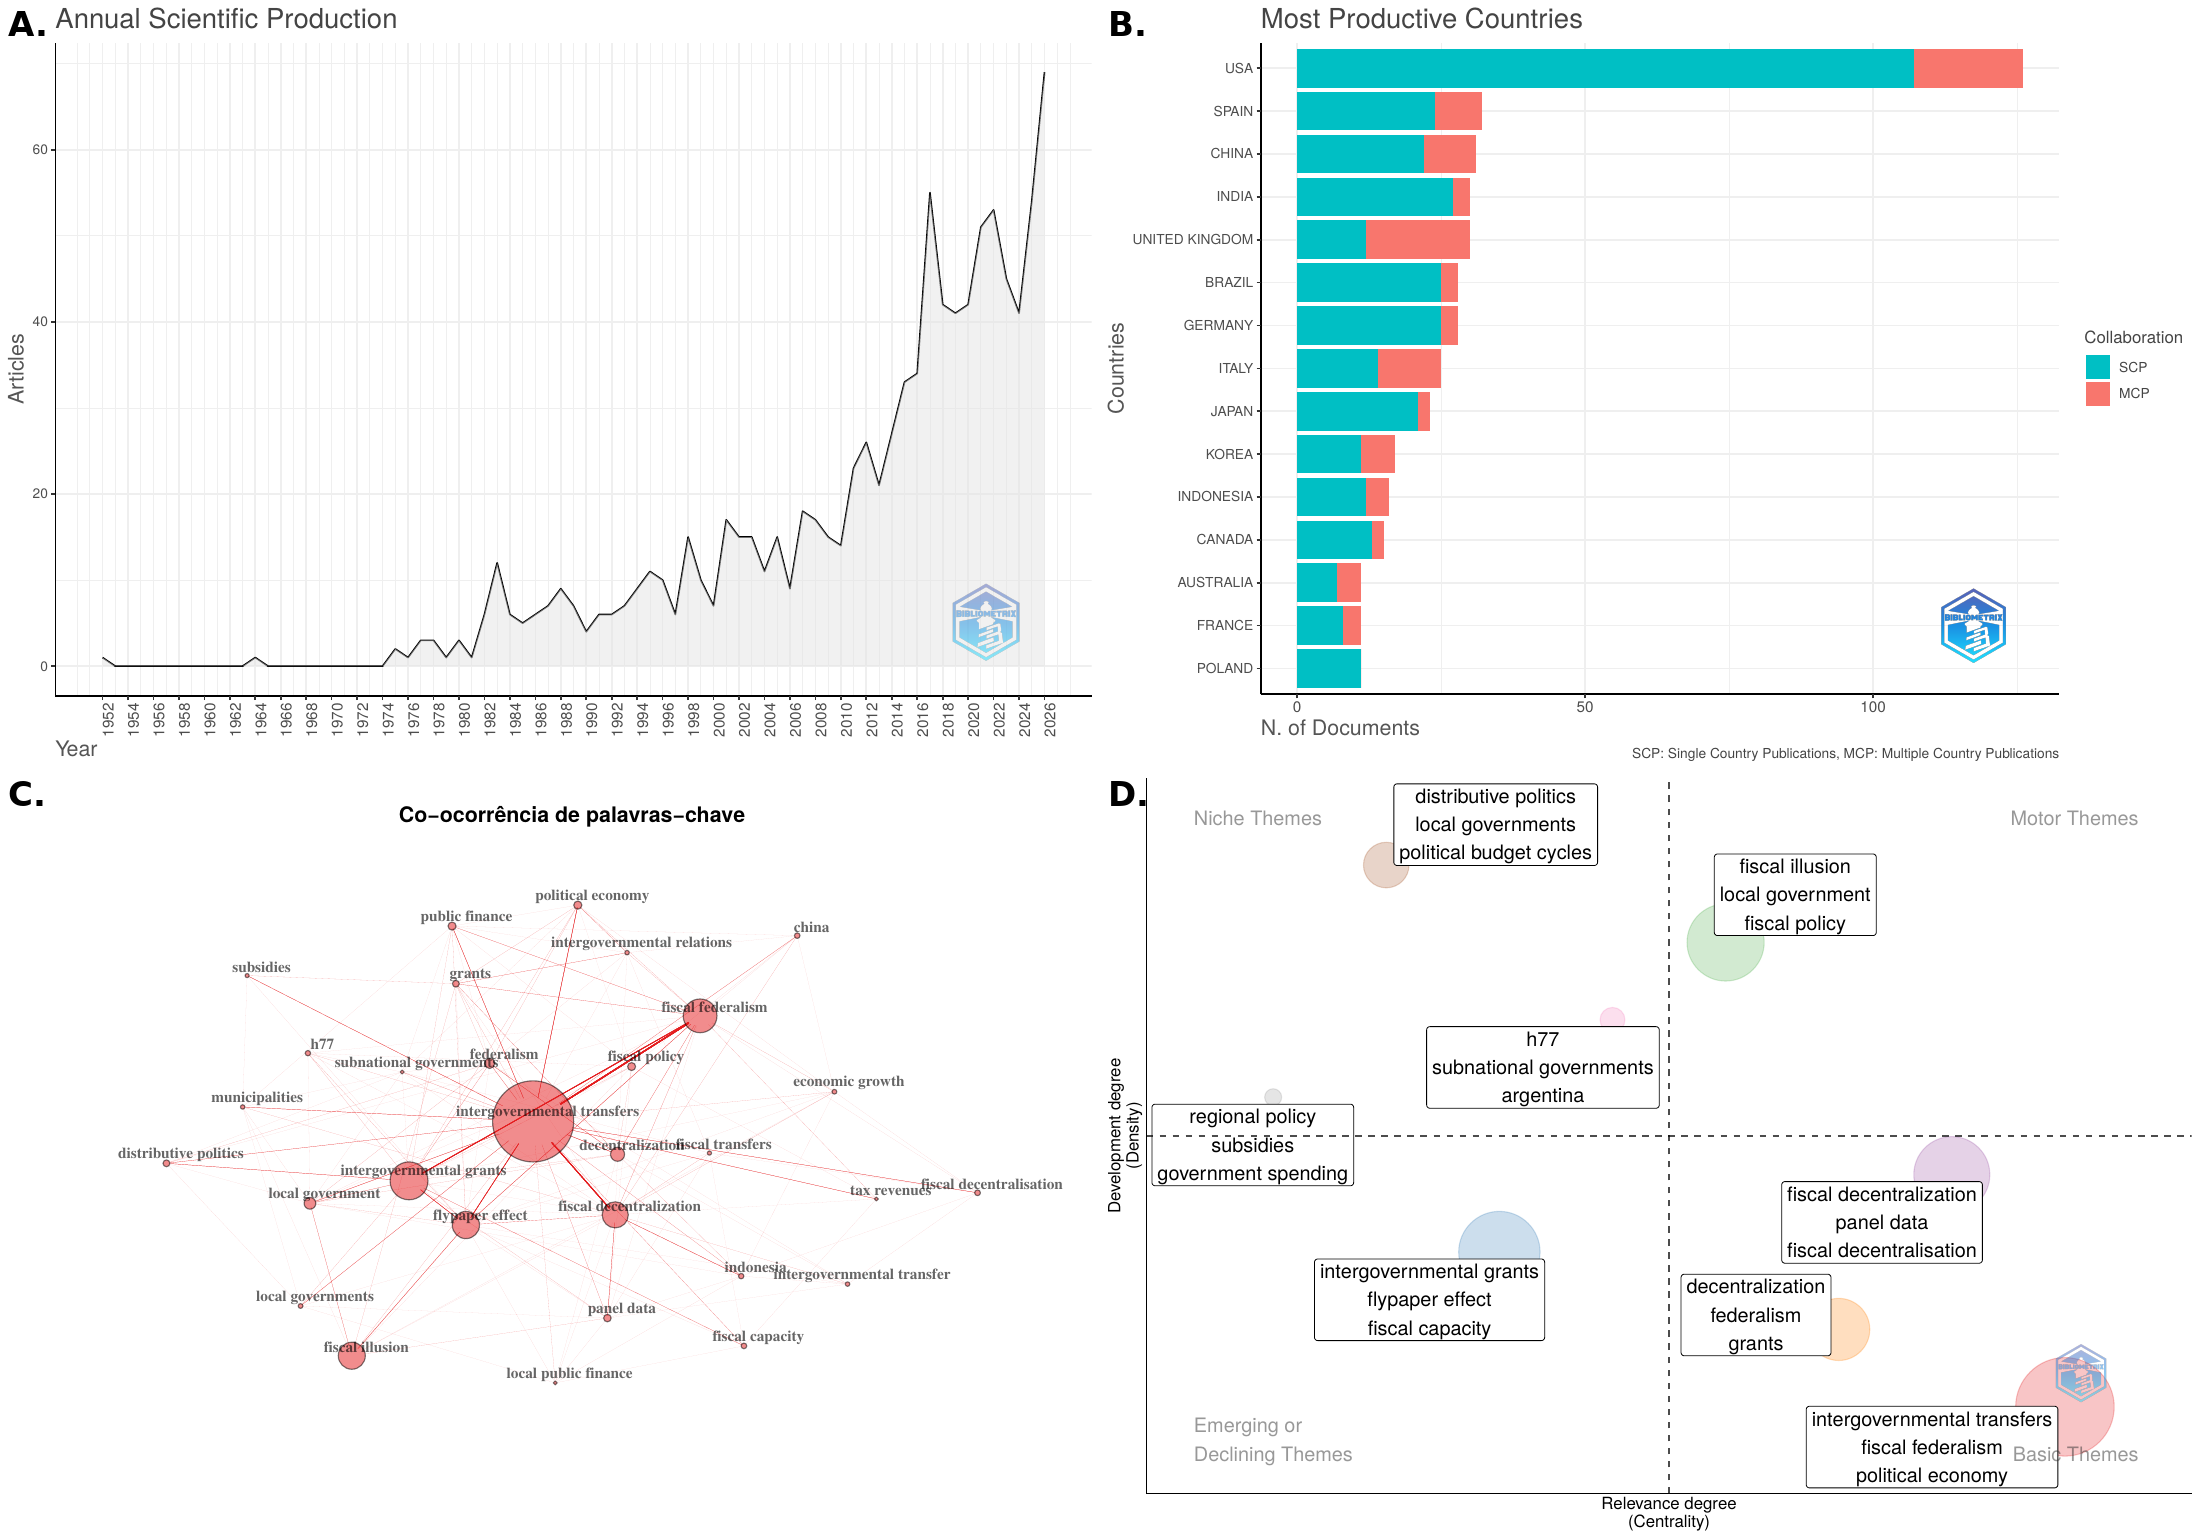
\includegraphics[width=0.92\textwidth]{../output/bibliometrix_painel.png}
\caption{Estudo bibliométrico com o \textit{bibliometrix} (968 artigos e revisões do Scopus, 1952--2026). A: produção científica anual; B: países mais produtivos (SCP: coautoria só do país; MCP: coautoria internacional); C: co-ocorrência de palavras-chave dos autores; D: mapa temático. Fonte: exportação do Scopus de 23/10/2026; cálculo do autor com o \textit{bibliometrix}.}\label{fig:biblio}
\end{figure*}

\noindent Dos 968 documentos foram selecionados, por leitura dos resumos, 80 artigos para o referencial, distribuídos nos cinco eixos da Tabela~\ref{tab:refs}. A seleção priorizou aderência temática (descartei, por exemplo, usos de \textit{flypaper} em finanças de carteira e em microempresas) e cobertura de períodos e países. Cada artigo tem DOI e a lista completa está em \texttt{docs/referencias\_80.csv}. Como a exportação traz os resumos, mas não o texto integral, a discussão a seguir se limita ao que os resumos permitem afirmar.

\begin{table}[t]
\centering\footnotesize
\caption{Os 80 artigos do referencial por eixo temático e período de publicação.}\label{tab:refs}
\setlength{\tabcolsep}{2.5pt}
\resizebox{\columnwidth}{!}{\begin{tabular}{p{3.1cm}rrrrrr}
\toprule
Eixo & $\le$1989 & 1990s & 2000s & 2010s & 2020s & Total\\
\midrule
Efeito flypaper & 3 & 7 & 6 & 5 & 0 & 21\\
Ilusão fiscal & 2 & 4 & 6 & 1 & 0 & 13\\
Brasil & 0 & 0 & 3 & 7 & 7 & 17\\
América Latina e em desenvolvimento & 0 & 1 & 4 & 8 & 5 & 18\\
Economia política e desempenho & 0 & 3 & 6 & 1 & 1 & 11\\
\midrule
Total & 5 & 15 & 25 & 22 & 13 & 80\\
\bottomrule
\end{tabular}}

\vspace{2pt}{\scriptsize Nota: os 80 artigos aparecem em 47 periódicos; a mediana de citações no Scopus é 48. Fonte: Scopus; cálculo do autor.}
\end{table}

\section{Referencial teórico e hipóteses}\label{sec:teoria}

\subsection{O enigma do flypaper}
O ponto de partida é uma anomalia: em teoria, uma transferência de montante fixo equivale a um aumento de renda dos residentes, mas o gasto local responde mais à primeira. \citet{bailey1998} fazem uma revisão ampla e concluem que a literatura, quase toda neoclássica, trouxe contribuições apenas marginais nos trabalhos mais recentes e que há caminhos de pesquisa mais produtivos. As explicações podem ser agrupadas em três famílias.

A primeira trabalha com maximização de bem-estar e dispensa o comportamento oportunista. \citet{hamilton1983} propõe um modelo em que a renda própria entra como insumo na produção de serviços locais; como ela substitui insumos comprados, a propensão a gastar em insumos é menor com renda própria do que com transferências. \citet{hamilton1986} mostra que o custo marginal crescente dos impostos explica a diferença, sem exigir burocracia estratégica ou erro de percepção dos eleitores, e \citet{dahlby2011} acrescenta que a transferência permite reduzir a alíquota e, assim, o custo marginal dos fundos públicos, um efeito-preço além do efeito-renda. \citet{vegh2015}, com as províncias argentinas de 1963 a 2006, atribuem o flypaper à resposta diferente da poupança precaucional a choques de renda e de transferências, e preveem que o efeito diminui com a correlação entre os dois.

A segunda família envolve informação e política. \citet{turnbull1992,turnbull1998} tratam eleitores racionais que decidem sob incerteza ou informação imperfeita, e mostram que cada tipo de imperfeição modifica o superdispêndio e o flypaper previstos pelo modelo de certeza. \citet{dougan1988} explicam o fenômeno por \textit{lobbying} de grupos de interesse, sem ilusão fiscal, e preveem variação do efeito entre categorias de despesa. \citet{leduc2017} acham que os estados dos EUA gastaram mais do que um dólar por dólar de repasse rodoviário em 2009--2011 e ligam o resultado a contribuições políticas do setor de obras. \citet{bracco2015} mostram que o alinhamento partidário entre níveis de governo afeta os repasses e as eleições, e \citet{volden2007} modela as decisões nacionais e subnacionais de forma conjunta, o que ajuda a entender por que estudos que as separam ficam incompletos.

A terceira família questiona a medida. \citet{becker1996} defende que o flypaper pode ser artefato de forma funcional, e \citet{wyckoff1991} testa quatro explicações conhecidas com escolas de Michigan e não confirma nenhuma. \citet{knight2002} argumenta que o repasse é endógeno, pois grants correlacionam com a preferência por bens públicos, e que o uso de instrumentos de poder político produz um efeito de substituição relevante. \citet{allers2016} usam uma reforma holandesa e mostram que o aumento de transferências foi capitalizado nos preços dos imóveis, o que torna improvável a explicação por \textit{rent seeking} de políticos ou burocratas. \citet{strumpf1998} sugere que o flypaper deve ser mais forte onde os gastos administrativos são altos, sinal de menor controle dos eleitores.

\subsection{Ilusão fiscal}
\citet{dollery1996} reúnem cinco hipóteses sob o rótulo de ilusão fiscal: complexidade da receita, elasticidade da receita, flypaper, ilusão do locatário e ilusão da dívida. Os testes empíricos são heterogêneos. Há apoio em 110 cidades suíças \citep{pommerehne1978} e em 302 municípios flamengos \citep{heyndels1994}; \citet{grossman1990} acha que transferências federais estimulam mais o gasto do que as estaduais em Virgínia, como previsto se a ilusão cresce com a separação entre quem tributa e quem gasta. \citet{sausgruber2005} testam em laboratório a hipótese de Mill e mostram que o tributo indireto é subestimado e distorce a decisão, embora os eleitores aprendam com o tempo; \citet{winter2001} encontram ilusões assimétricas, em que usuários e produtores de serviços são mais favoráveis ao gasto do que o contribuinte comum. Por outro lado, \citet{misiolek1988} acham pouca evidência de ilusão fiscal, e \citet{carroll2009} não a encontram em municípios americanos, embora a diversificação da receita afete a volatilidade; \citet{hendrick2002} associam maior diversificação a menor esforço tributário. \citet{campbell2004} mostram que ignorar a relação vertical entre jurisdições sobrepostas superestima os efeitos horizontais, e \citet{dellanno2014} constroem um índice de ilusão fiscal para 28 países europeus. \citet{ashworth1997} usam a opinião de políticos locais para testar indiretamente hipóteses de escolha tributária, e \citet{mcgillivray2001} estendem a lógica à ajuda externa, em que o gasto agregado sobe mais do que a ajuda recebida. \citet{arvate2009}, com eleições estaduais no Brasil, não encontram evidência de ilusão fiscal na reação dos eleitores a superávits.

\subsection{Assimetria e pegajosidade}
Uma segunda pergunta é se o gasto cai tanto quanto sobe. \citet{gamkhar1996} não encontram assimetria nos dados agregados dos EUA e concluem que o flypaper opera nos dois sentidos. Outros estudos acham o contrário. Em municípios flamengos, \citet{heyndels2001} observa que o gasto não cai com cortes de transferências e que a perda é compensada com impostos, ou seja, substituição fiscal; \citet{deller2006} chegam à mesma conclusão com o programa de receitas compartilhadas de Wisconsin, e \citet{shani2023}, com uma reforma israelense, mostram que cortes elevaram alíquotas locais e déficits. \citet{dash2013} testam a hipótese de assimetria nos estados indianos e acham arrecadação inversamente relacionada a transferências não condicionadas, em aumentos e em quedas. \citet{volden1999} estuda os programas de assistência a famílias e mostra respostas assimétricas que dependem de pressões burocráticas e políticas. \citet{levaggi2003} examinam o mesmo problema na saúde das regiões italianas, e \citet{melo2002} acha, na Colômbia, que o flypaper aparece onde os entes dependem muito de transferências, e analisa assimetrias na resposta às transferências conforme o grau de dependência.

\subsection{Transferências e esforço fiscal}
Se a transferência substitui a arrecadação, o município se acomoda. \citet{baretti2002} encontram na Alemanha que transferências equalizadoras reduzem a receita tributária dos estados, e \citet{kalb2010} associam mais transferências a maior folga organizacional nos municípios alemães. \citet{dahlberg2008} usam uma descontinuidade na regra de repasse sueca e acham que as transferências aumentam o gasto local sem reduzir as alíquotas. Em países em desenvolvimento, os resultados variam: \citet{mogues2012} mostram que, em Gana, o conjunto das transferências desestimula a receita interna, e \citet{masaki2018} faz a mesma pergunta para a Tanzânia. \citet{aragon2013}, no Peru, acham que o efeito das transferências sobre o gasto é maior onde cobrar tributos localmente é mais caro, e \citet{porto2023}, em Buenos Aires, acham que as transferências \textit{facilitam} a arrecadação própria e a deslocam para o IPTU. \citet{lewis2017} encontram apoio apenas misto aos incentivos perversos atribuídos ao sistema indonésio, e \citet{zhang2013} separa, na China, o efeito de repasses de partilha tributária, gerais e específicos. No Brasil, \citet{litschig2013} acham que repasses extras elevaram o gasto \textit{per capita} em cerca de 20\% sem evidência de substituição da receita própria, e \citet{mattos2011} propõem que repasses maiores reduzem a eficiência da arrecadação. \citet{alves2024} usam as faixas de população do FPM para testar incentivos locais.

\subsection{Evidências brasileiras}
\citet{araujo2016} estimam a demanda por gastos locais para 5.249 municípios em 2010 e atribuem à dependência de transferências e à opacidade tributária a chance de ilusão fiscal. \citet{ferreira2019} mostram flypaper em 476 municípios, que se intensifica com o alinhamento político, e usam o alinhamento como instrumento. \citet{castro2021} explicam cerca de 20\% do flypaper pelas transferências dos municípios vizinhos. \citet{cruz2020} estudam a regra de gasto mínimo em educação, e \citet{mattos2018} mostram que repasses em bloco aumentam a dispersão do gasto em educação, ao contrário dos categóricos. \citet{bernardo2020} associam as transferências e o FUNDEB à qualidade da educação nas regiões Norte e Nordeste, e \citet{decarvalhofilho2020} mostram que o aumento temporário de transferências nos anos 1980 teve efeitos que persistem até os anos 2000. Em nível estadual, \citet{prado2020} encontram evidências de ilusão fiscal causada por déficit e por transferências, e possíveis efeitos flypaper, mas não da lei de Wagner, e \citet{marconi2009} mostram que parte das transferências é apropriada pela burocracia em forma de salários. \citet{neto2013} e \citet{brollo2012} tratam a alocação: \citet{brollo2012} mostram que prefeitos alinhados à coalizão do presidente recebem cerca de um terço mais em transferências discricionárias para infraestrutura nos anos pré-eleitorais, e \citet{ferreira2021} estendem a análise para 2.856 municípios, em que o alinhamento com o governo federal e a troca de favores no Congresso importam.

\subsection{Economia política das transferências}
A alocação não é neutra. \citet{grossman1994} formula uma teoria política em que políticos federais compram o apoio de eleitores e políticos estaduais; \citet{johansson2003} mostram transferências táticas na Suécia, e \citet{soleolle2008} identificam o efeito do alinhamento partidário na Espanha. \citet{treisman1996} analisa o caso russo pós-soviético, \citet{veiga2007} o português, \citet{porto2001} e \citet{bonvecchi2011} o argentino (neste, repasses discricionários e não discricionários dão retorno político distinto), \citet{mejiaacosta2019} o equatoriano e \citet{bastida2022} o hondurenho, onde o flypaper e o partidarismo explicam bem o desempenho financeiro. \citet{gainza2021} comparam Brasil, México, Colômbia e Chile e acham manipulação do ciclo eleitoral e viés para municípios alinhados, com diferenças entre países. No plano das instituições, \citet{rodden2002} associa déficits subnacionais persistentes à combinação de dependência de transferências e liberdade de endividamento, e \citet{sanguinetti2004} analisam a troca entre seguro e disciplina agregada em arranjos de transferência.

\subsection{Países em desenvolvimento e Ásia}
\citet{bird2002} resumem as lições internacionais: as transferências devem dar a quem as recebe mandato claro, recursos adequados, flexibilidade e prestação de contas. \citet{bahl1994} mostram que países em desenvolvimento têm estruturas fiscais mais centralizadas e usam uma variedade de instrumentos de transferência com graus distintos de controle do centro. \citet{tsui2005} decompõem as disparidades fiscais dos condados chineses, \citet{aritenang2020} mostram que as transferências são a fonte principal do gasto de capital dos distritos indonésios, e \citet{guerrero2022} propõem um modelo para a realocação de transferências entre estados mexicanos. \citet{vandewalle2007} encontram flypaper em ajuda a projetos rurais no Vietnã, e \citet{masaki2018} acentua que a capacidade fiscal local na África subsaariana é limitada. Esses trabalhos ajudam a ler a Malásia como uma federação de renda média com forte centro, embora sem estudo direto na nossa base.

\subsection{Hipóteses}
O referencial gera hipóteses testáveis com o painel do Amazonas, em que $G$ é o gasto corrente, $T$ as transferências, $Y$ o PIB \textit{per capita} (proxy da renda local) e $R^p$ a receita própria corrente:
\begin{itemize}\setlength{\itemsep}{0pt}
\item \textbf{H1 (flypaper).} $\beta_T>\beta_Y>0$: o gasto responde mais às transferências do que à renda.
\item \textbf{H2 (assimetria/pegajosidade).} $\beta^{+}>\beta^{-}$: o gasto sobe com aumentos das transferências mais do que cai com reduções.
\item \textbf{H3 (substituição fiscal).} A elasticidade da receita própria às transferências é negativa.
\item \textbf{H4 (FUNDEB).} O resultado de H1 não depende do FUNDEB, que é vinculado, ao contrário das transferências livres.
\end{itemize}

\section{Dados e métodos}\label{sec:dados}

\subsection{Base de dados}
A base cobre 2014--2023, os dez anos mais recentes com PIB municipal divulgado. As receitas e despesas vêm do Finbra/Siconfi (Contas Anuais, anexos I-C e I-D, \textit{Municípios do Estado -- AM}), o PIB e o valor adicionado do IBGE, e o deflator do IPCA dezembro a dezembro (Ipeadata). Os valores são expressos em reais de 2023 e por habitante. As regras que valem para toda a base: lacuna é dado ausente, nunca zero; o zero de receita de capital só é aceito quando o total oficial o comprova (46 observações, nenhuma focal); e a conferência entre componentes e total oficial de receitas fecha em 609 das 609 observações com dados (diferença menor que R\$ 1). O painel tem 620 linhas (62 municípios $\times$ 10 anos), das quais 609 têm receitas; Tabatinga não consta nos arquivos do Siconfi em 2015 e 2016. O plano de contas de receitas mudou duas vezes no período (A: 2014--17; B: 2018--21; C: 2022--23), tratado por código normalizado. A receita total exclui as receitas intraorçamentárias nos três planos, e o total de transferências substitui a divisão União/Estados, que não é comparável entre planos. O dicionário (\texttt{docs/dicionario\_variaveis.csv}, 98 variáveis) e o registro de alterações (\texttt{docs/registro\_alteracoes.md}) detalham fonte, unidade, tratamento e fórmula de cada variável.

Para a Malásia, usei o Banco Mundial (WDI), com as séries de governo \textit{central} (receita, tributos, despesa, saldo e dívida em \% do PIB), e o FMI (WEO 9.0.0), em governo \textit{geral}, para 2014--2024; os valores reais usam o IPC do WDI com base em 2023. Lacunas são mantidas (a despesa do governo central em 2024 está ausente). Não há dado malaio de transferências a estados ou governos locais no período; as fontes possíveis (Ministry of Finance, DOSM, Bank Negara Malaysia) são citadas no código de coleta, mas não foram coletadas, e isso restringe a comparação.

\subsection{Modelos}
Os modelos de painel usam efeitos fixos de município $\alpha_i$ e de ano $\lambda_t$, com variáveis em logaritmos. A equação central de H1 é
\begin{equation}
\ln G_{it}=\alpha_i+\lambda_t+\beta_T\ln T_{it}+\beta_Y\ln Y_{it}+\varepsilon_{it},
\end{equation}
com sinais esperados $\beta_T>0$, $\beta_Y>0$ e $\beta_T>\beta_Y$. Os modelos M2--M7 e M10--M12 usam essa forma, trocando a variável dependente (receita própria, receita tributária, despesa de pessoal, investimento) ou a amostra; M1 substitui $Y$ por $R^p$. Para H3, a variável dependente é $\ln R^{p}_{it}$ e $\beta_T<0$ indica substituição. Para H2, a equação em primeira diferença, que elimina $\alpha_i$, é
\begin{equation}
\Delta\ln G_{it}=\lambda_t+\beta^{+}\Delta^{+}\ln T_{it}+\beta^{-}\Delta^{-}\ln T_{it}+\gamma\,\Delta\ln Y_{it}+u_{it},
\end{equation}
em que $\Delta^{+}=\max(\Delta\ln T,0)$ e $\Delta^{-}=\min(\Delta\ln T,0)$. Como $\Delta^{-}\le 0$, um $\beta^{-}>0$ significa que o gasto cai quando a transferência cai; simetria é $\beta^{+}=\beta^{-}$ e pegajosidade é $\beta^{-}<\beta^{+}$. Para H4, repete-se (1) com as transferências sem o FUNDEB.

A estimação usa a transformação \textit{within} por município, com dummies de ano, por MQO, e erros-padrão robustos agrupados por município (62 \textit{clusters}), que toleram heterocedasticidade e autocorrelação serial dentro do município. As variáveis dependentes e explicativas em $\ln$ exigem valores positivos; observações com valor ausente ou não positivo saem da amostra de cada modelo. A elasticidade-PIB é uma \textit{proxy} imperfeita da renda dos residentes, pois o PIB municipal do Amazonas contém muita administração pública, financiada por transferências. Os diagnósticos reportados são o $R^2$ \textit{within}, o número de observações e municípios, a correlação entre $\ln T$ e $\ln Y$ (0,29, sem colinearidade grave) e os testes de robustez M10 (apenas 2014--2021, planos A e B), M11 (sem 1\% maiores transferências \textit{per capita}) e M12 (sem os dois focais). Os efeitos fixos controlam diferenças permanentes entre municípios, mas não resolvem a endogeneidade das transferências, e por isso os coeficientes são lidos como associações. Não há instrumentos: o painel não inclui dados eleitorais, como os de alinhamento usados por \citet{ferreira2019}.

\section{Resultados}\label{sec:res}

\subsection{Descrição}
A Figura~\ref{fig:desc} e a Tabela~\ref{tab:desc} mostram os casos focais. As transferências \textit{per capita} subiram em todo o Amazonas a partir de 2017. Em Tabatinga elas saltaram de R\$ 2,5 mil em 2018 para R\$ 4,4 mil em 2023, e em Humaitá de R\$ 2,6 mil para R\$ 3,7 mil. Em 2018 e 2023 a dependência de transferências fica abaixo da mediana estadual nos dois municípios (87--93\% contra 95\%), porque a arrecadação própria corrente \textit{per capita} é maior que a mediana: R\$ 391 e R\$ 576 em 2023, contra R\$ 273. Em 2023 Tabatinga gasta mais por habitante com pessoal (R\$ 2.288) e investimento (R\$ 673) do que Humaitá (R\$ 1.725 e R\$ 282); a mediana estadual é R\$ 2.189 e R\$ 545. O FUNDEB \textit{per capita} aumenta de 2021 para 2022 nos dois, mas essa alta coincide com a mudança do plano de contas e com a nova complementação, e não pode ser lida como choque puro.

\begin{table}[t]
\centering\footnotesize
\caption{Casos focais e mediana dos 62 municípios do AM (R\$ de 2023 \textit{per capita}).}\label{tab:desc}
\setlength{\tabcolsep}{3.5pt}
\begin{tabular}{llrrrr}
\toprule
Ano & Unidade & Transf. & Rec. própria & Dep. (\%) & Gasto corr.\\
\midrule
2014 & Tabatinga & 2.404 & 88 & 96 & 1.929\\
 & Humaitá & 2.695 & 228 & 92 & 2.511\\
 & Mediana AM & 2.996 & 132 & 96 & 2.550\\
2018 & Tabatinga & 2.475 & 188 & 93 & 2.088\\
 & Humaitá & 2.611 & 314 & 89 & 2.511\\
 & Mediana AM & 3.037 & 152 & 95 & 2.737\\
2023 & Tabatinga & 4.436 & 391 & 92 & 3.653\\
 & Humaitá & 3.728 & 576 & 87 & 3.681\\
 & Mediana AM & 4.846 & 273 & 95 & 4.094\\
\bottomrule
\end{tabular}

\vspace{2pt}{\scriptsize Nota: ``Dep.'' é transferências totais sobre receita total, sem receitas intraorçamentárias. Fonte: Finbra/Siconfi, IBGE, IPCA; cálculo do autor.}
\end{table}

\begin{figure*}[t]
\centering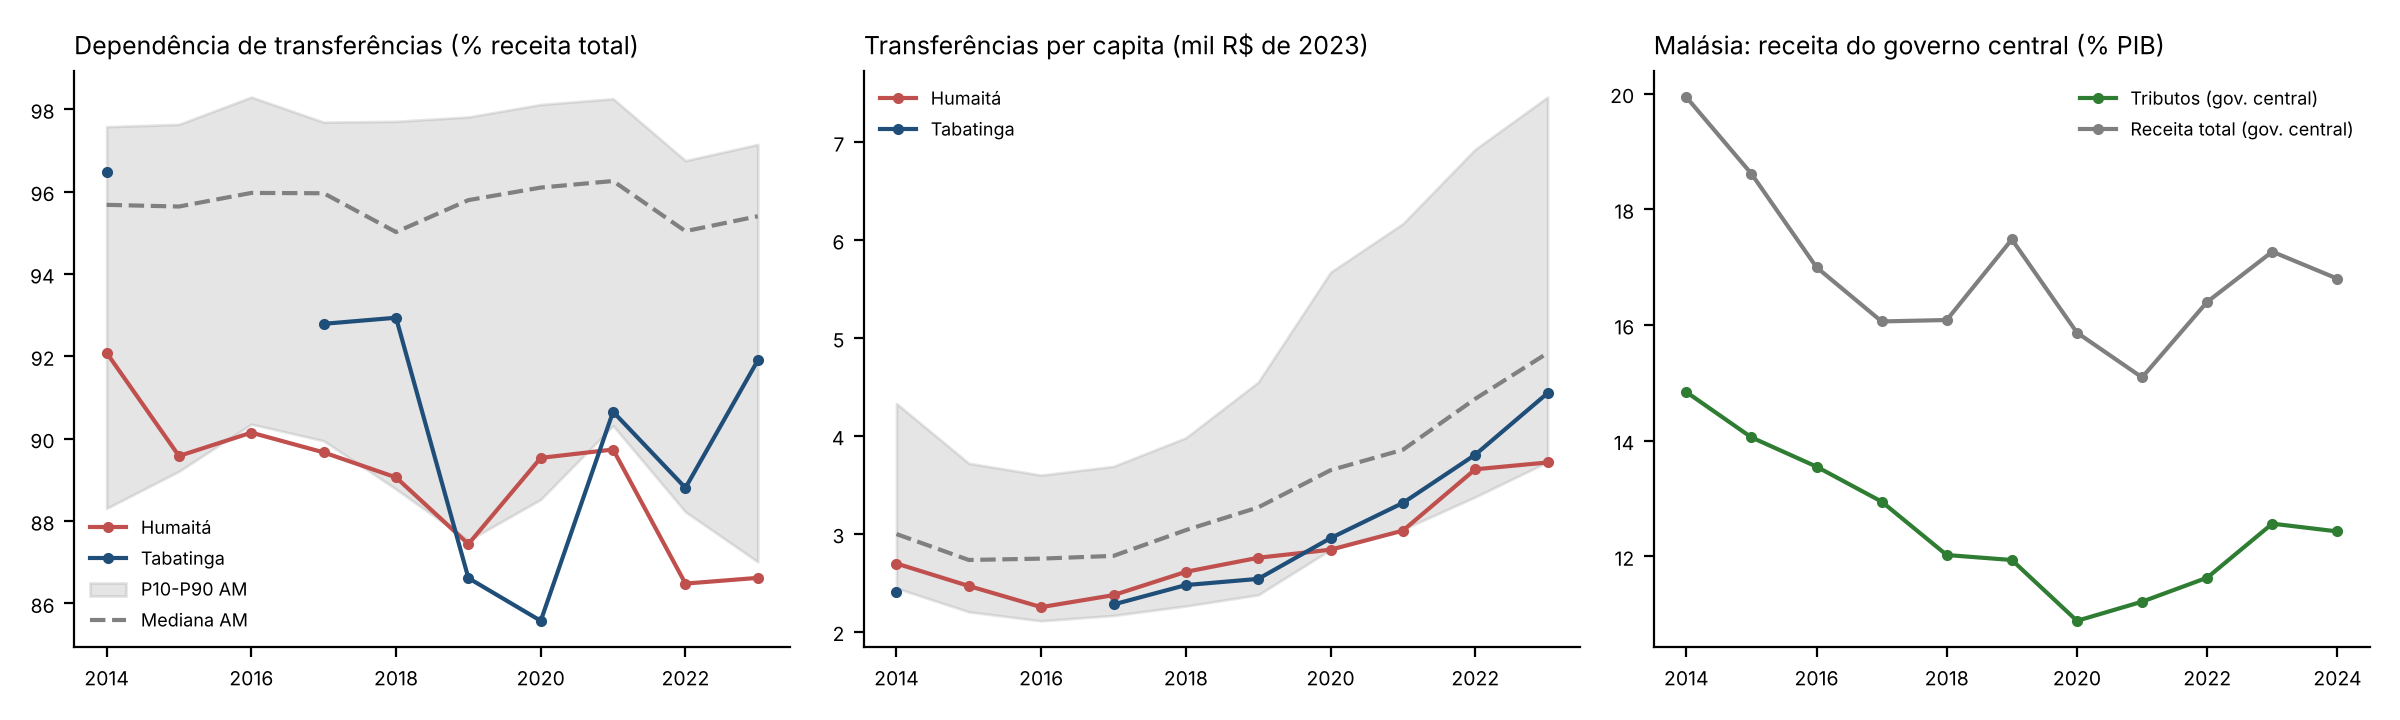
\includegraphics[width=0.95\textwidth]{../output/fig_descritivas.png}
\caption{Esquerda e centro: dependência de transferências e transferências \textit{per capita} reais de Tabatinga e Humaitá, com mediana e intervalo P10--P90 dos 62 municípios (Tabatinga sem dados em 2015 e 2016). Direita: receita total e tributos do governo central da Malásia em \% do PIB. Fonte: Finbra/Siconfi, Banco Mundial; cálculo do autor.}\label{fig:desc}
\end{figure*}

\subsection{Flypaper e esforço fiscal no Amazonas}
A Tabela~\ref{tab:reg} resume as estimações. Em M2, uma elevação de 10\% nas transferências \textit{per capita} se associa a 5,3\% mais gasto corrente, enquanto 10\% mais PIB \textit{per capita} se associa a 1,8\% (p = 0,025). O resultado sustenta H1 pelo critério da razão entre elasticidades, cerca de três vezes. Há, porém, duas ressalvas. Primeiro, elasticidades não são propensões marginais a gastar. Multiplicando cada elasticidade pela razão mediana entre gasto e a base correspondente (0,87 para as transferências e 0,24 para o PIB \textit{per capita}), as propensões implícitas seriam de cerca de 0,46 e 0,04; a diferença seria ainda maior, mas essa conversão é aproximada e não foi estimada diretamente. Segundo, o PIB municipal inclui a administração pública e não equivale à renda dos moradores. Quando as transferências excluem o FUNDEB (M3) o coeficiente é 0,51, e não 0,53, o que sustenta H4: a vinculação ao fundo não gera o resultado. A exclusão dos dois focais (M12) deixa tudo praticamente igual, e a exclusão dos 1\% maiores valores (M11) reduz a elasticidade-transferência a 0,46 e a elasticidade-PIB a 0,10 (p = 0,07).

\begin{table*}[t]
\centering\footnotesize
\caption{Painel dos municípios do Amazonas, 2014--2023: efeitos fixos de município e de ano, erros-padrão agrupados por município entre parênteses.}\label{tab:reg}
\begin{tabular}{llcccccc}
\toprule
Modelo & Variável dependente & $\ln T$ & $\ln T$ s/ FUNDEB & $\ln Y$ & $\ln R^p$ & $N$ & $R^2_w$\\
\midrule
M1 & $\ln$ gasto corrente & 0,559*** \ep{0,132} & & & 0,066*** \ep{0,020} & 609 & 0,851\\
M2 & $\ln$ gasto corrente & 0,534*** \ep{0,102} & & 0,179** \ep{0,080} & & 609 & 0,849\\
M3 & $\ln$ gasto corrente & & 0,512*** \ep{0,075} & 0,206** \ep{0,083} & & 609 & 0,846\\
M4 & $\ln$ receita própria corrente & 0,659*** \ep{0,188} & & 0,183 \ep{0,134} & & 609 & 0,343\\
M5 & $\ln$ receita tributária & 0,463*** \ep{0,176} & & 0,181 \ep{0,156} & & 609 & 0,388\\
M6 & $\ln$ despesa de pessoal & 0,386*** \ep{0,091} & & 0,267*** \ep{0,083} & & 609 & 0,751\\
M7 & $\ln$ investimento & 1,602*** \ep{0,444} & & $-0{,}629$** \ep{0,273} & & 609 & 0,405\\
M10 & gasto corrente, 2014--21 & 0,392*** \ep{0,099} & & 0,118 \ep{0,095} & & 485 & 0,695\\
M11 & gasto corrente, sem 1\% maiores $T$ & 0,462*** \ep{0,089} & & 0,098* \ep{0,054} & & 602 & 0,838\\
M12 & gasto corrente, sem focais & 0,533*** \ep{0,102} & & 0,180** \ep{0,081} & & 591 & 0,847\\
\bottomrule
\end{tabular}

\vspace{2pt}{\scriptsize Nota: *** p<0,01, ** p<0,05, * p<0,10. Todas as variáveis em $\ln$ de R\$ de 2023 \textit{per capita}; $T$ = transferências totais, $Y$ = PIB \textit{per capita}, $R^p$ = receita própria corrente. $R^2_w$ = $R^2$ \textit{within}. Fonte: cálculo do autor (\texttt{R/07\_regressoes.py}).}
\end{table*}

Sobre H3, M4 e M5 mostram o contrário da substituição: receita própria e tributária \textit{crescem} com as transferências (0,66 e 0,46). Isso lembra o resultado de \citet{porto2023} para Buenos Aires e o de \citet{litschig2013} para o Brasil, e contraria Gana, Tanzânia e Alemanha \citep{mogues2012,masaki2018,baretti2002}. A leitura prudente é que a correlação positiva reflete movimentos comuns (a estrutura econômica e o tamanho do município podem aumentar as duas), e não que a transferência estimule arrecadação; a receita própria é pequena, e variações percentuais sobre bases pequenas são grandes. Em M7, o investimento responde muito às transferências (1,60), e o gasto de pessoal bem menos (0,39), um padrão compatível com a ideia de que transferências financiam obras, embora o investimento seja volátil e o $R^2$ seja baixo.

\subsection{Assimetria}
A Tabela~\ref{tab:asym} mostra M8 e M9 em primeira diferença. O gasto corrente sobe 0,21 para cada 1 de aumento logarítmico das transferências (p = 0,005) e cai apenas 0,08 para cada 1 de queda (p = 0,30). A direção é a de H2, mas o teste de igualdade $\beta^{+}=\beta^{-}$ tem $z=1{,}39$ (p = 0,165). A evidência de pegajosidade é, portanto, sugestiva e não conclusiva, e o mesmo vale para a leitura de substituição fiscal, de \citet{heyndels2001} e \citet{deller2006}: em M9, nenhum dos dois coeficientes é distinguível de zero. O contraste com \citet{gamkhar1996}, que não acham assimetria, não pode ser resolvido com 540 observações e dez anos. Há outro motivo de cautela: o período inclui a pandemia e a mudança do FUNDEB, e a variação em $\ln T$ é grande em 2022.

\begin{table}[t]
\centering\footnotesize
\caption{Assimetria (primeira diferença, efeitos fixos de ano, EP agrupados).}\label{tab:asym}
\setlength{\tabcolsep}{4pt}
\begin{tabular}{lcc}
\toprule
& M8: $\Delta\ln G$ & M9: $\Delta\ln R^p$\\
\midrule
$\Delta^{+}\ln T$ ($\beta^{+}$) & 0,211*** \ep{0,074} & 0,206 \ep{0,206}\\
$\Delta^{-}\ln T$ ($\beta^{-}$) & 0,078 \ep{0,075} & 0,016 \ep{0,250}\\
$\Delta\ln Y$ & $-0{,}021$ \ep{0,097} & 0,207 \ep{0,240}\\
$N$ / $R^2_w$ & 540 / 0,386 & 540 / 0,116\\
$H_0$: $\beta^{+}=\beta^{-}$ & $z=1{,}39$ (p = 0,165) & ---\\
\bottomrule
\end{tabular}
\end{table}

\subsection{Tabatinga e Humaitá em relação ao estado}
Os dois focais ficam, na maior parte dos anos, dentro do intervalo P10--P90 do estado em transferências \textit{per capita}, e em alguns anos (Tabatinga em 2020; Humaitá em 2022--23) abaixo do P10 em dependência. O que os distingue é a receita própria maior que a mediana e a trajetória: Tabatinga, que tinha a menor arrecadação própria \textit{per capita} entre os dois em 2014 (R\$ 88), mais que quadruplica até 2023 (R\$ 391). Como o modelo tem efeitos fixos, essas diferenças de nível não afetam os coeficientes; os focais não alteram o resultado (M12). A leitura causal de por que a arrecadação própria cresceu mais que o estado exigiria dados que a base não tem, como o cadastro imobiliário ou a atividade econômica de fronteira.

\subsection{Malásia como contraponto}
A comparação com a Malásia é institucional e descritiva. Os países diferem em moeda, escala e organização federativa, e os dados são de governo central, não subnacional, então não se compara nível com nível. O governo central malaio arrecadou tributos equivalentes a 14,8\% do PIB em 2014, cifra que cai para 10,9\% em 2020 e recupera para 12,4\% em 2024; a receita total foi de 19,9\% para 15,1\% (2021) e 16,8\% (2024). A dívida do governo central subiu de 52,7\% para 64,6\% do PIB, e a despesa do governo geral (WEO) ficou em 22,0--26,0\%. O PIB \textit{per capita} real cresceu de MYR 42,5 mil para 53,4 mil (2023). Dois pontos importam para a leitura do Amazonas. Primeiro, o ente central malaio financia a si mesmo com tributos de 11--15\% do PIB, enquanto um município amazônico financia 87--97\% do orçamento com recursos de outros níveis: a pergunta do flypaper não se aplica ao centro, mas ao desenho de repasses. Segundo, a literatura sobre a Ásia mostra que o resultado depende do desenho: na China, os tipos de repasse têm efeitos distintos \citep{zhang2013,tsui2005}, e na Indonésia as transferências são o principal financiamento do gasto de capital distrital \citep{aritenang2020,lewis2017}. Um teste malaio exigiria dados de subvenções federais a estados e de receita estadual, que não foram obtidos.

\subsection{O que mudou em relação ao P1}
A base mudou de unidades (os dados disponíveis do P1 cobriam municípios do Rio de Janeiro e o Paraguai) e de escala (de 2 para 62 municípios). Foram tratadas as três versões do plano de contas, a receita total passou a excluir as intraorçamentárias, foram criados deflator e variáveis \textit{per capita}, e se acrescentou conferência automática contra o total oficial. O registro completo está em \texttt{docs/registro\_alteracoes.md}.

\section{Conclusão}\label{sec:conc}
Nos municípios do Amazonas entre 2014 e 2023, o gasto corrente responde bem mais às transferências do que ao PIB \textit{per capita}, e o resultado se mantém sem o FUNDEB, sem os casos focais e em subamostras. É a configuração prevista pela literatura do flypaper, que não distingue entre ilusão fiscal, custo marginal dos fundos, insumos de produção e política: o artigo não testa essas explicações entre si. O gasto sobe quando as transferências sobem e parece cair menos quando elas caem, mas a diferença não é estatisticamente significativa. Não há evidência de que as transferências substituam a receita própria.

As limitações são claras. Os coeficientes são associações condicionais; as transferências são endógenas e não há instrumentos, pois o painel não contém variáveis eleitorais. O PIB municipal é uma \textit{proxy} fraca da renda local; a população do Finbra repete valores em alguns anos; o deflator é dezembro a dezembro; os planos de contas mudam em 2018 e 2022; Tabatinga não aparece em 2015 e 2016. A parte da Malásia é descritiva, de governo central, sem dados subnacionais, e não há na base nenhum artigo sobre transferências aos estados malaios. Três passos naturais são incluir dados eleitorais para instrumentar as transferências, usar as faixas de população do FPM como descontinuidade, como fazem \citet{alves2024} e \citet{castro2021}, e obter os dados de subvenções a estados na Malásia.

\section*{Disponibilidade de dados e código}
Repositório com dados originais, brutos e tratados, dicionário, registro de alterações e \textit{scripts}: \url{https://github.com/JVContaifer/p2-financas-publicas-unb}. Fontes: Siconfi/Finbra (Tesouro Nacional), IBGE (PIB dos Municípios), Ipeadata (IPCA), Banco Mundial (WDI) e FMI (WEO 9.0.0).

\small
\bibliographystyle{plainnat}
\bibliography{refs}
\end{document}
